\title{Simulation using Hamiltonian Monte Carlo}
\author{
        Ho Chung Leon  Law \\
            \and
        Nathan Cunningham\\
}
\date{\today}

\documentclass[11pt]{article}
\usepackage{amsmath}
\usepackage{algorithm}
\usepackage{algpseudocode}
\usepackage{graphicx}
\usepackage{amssymb}
\usepackage{hyperref}
\usepackage[a4paper,bindingoffset=0.2in,%
            left=1in,right=1in,top=1in,bottom=1in,%
            footskip=.25in]{geometry}
\begin{document}
\maketitle

\begin{abstract}
In this report we aim to examine the properties of Hamiltonian Monte Carlo, implement it in the R coding language, and compare its effectiveness to another method of monte carlo simulation. \ldots
\end{abstract}
\newpage
\section{Introduction}
Some popular methods to simulate from a density of interest is to use Metropolis Hasting and Gibbs Sampling and very commonly a random walk proposal is used. However, these may have slow mixing properties in certain situations, especially in a high-dimensional setting. Hamiltonian Monte Carlo (HMC) on the other hand make use of the first-order gradient information of the target density, which then allows us to coherently explore the state space. This is done through the introduction of auxiliary momentum variables, which then allows us to use Hamiltonian dynamics  to then construct a ergodic markov chain, whose stationary distribution is our density of interest. 
\\
\\
In this report, we will to give a quick overview and intuition of the HMC algorithm, which is primarily based on Neal\cite{neal} and Duane et al\cite{duane} paper. We will then go on to implement the algorithm in R and compare results from different simulations using random walk Metropolis Hastings, HMC and No-U-Turn Sampler (NUTS). We will also illustrate these methods on mixture of gaussians, which resembles the 26 letters of the alphabets (Capital and Lower Case), where the parameters were found using EM-algorithm on an image data set of alphabets.
\section{Hamiltonian Monte Carlo}
\subsection{Target Density and Energy Function}
We first define our target density to be of the form (without normalising constant):
\begin{equation}
P(q)= \pi(q)L(q|D) \quad \quad q \in \mathbb{R}^{d}
\end{equation}
where $\pi(q)$ is the prior density and $L(q|D)$ is the likelihood given data $D$. But in generally clearly this can be any density.
We also define $q$ to be the 'position' vector in $d$ dimensions. Now, we note in statistical mechanics, given some energy function $E(x)$ via concept of the canonical distribution, we can express its canonical distribution as:
\begin{equation}
\label{energy}
Pr(x) = \frac{1}{Z}exp(-E(x)/T)
\end{equation}
where $T$ is the temperature of the system (which we can assume as 1) and $Z$ is a normalising constant. By considering this, we can now define the 'energy' of our target density as:
\begin{equation}
U(q) = -log[\pi(q)L(q|D)]
\end{equation}
We now introduce an auxiliary variable $p$ ('momentum' in $d$ dimensions), which we define to have energy function $K(p)$, which using equation \ref{energy} has in turns a density function $Q(p)$. We define the joint density of $(p,q)$ as 
\begin{equation}
P(q,p) = \frac{1}{Z}exp(-U(q)/T)exp(-K(p)/T) = \frac{1}{Z}exp(-H(q,p)/T)
\end{equation}
where $H(q,p) = U(q) + K(p)$ can be seen as the energy function for the joint state $(q,p)$.The independence of $q$ and $p$ allows easy extraction of samples from $P(q)$ and we remark that the introduction of $p$ enables us to use Hamiltonian Dynamics, which has very nice properties. 
\subsection{Hamiltonian dynamics}
Hamiltonian dynamics is the system described by a pair of differential equations with coordinates $(q,p)$, for $i=1 \dots d$
\begin{equation}
\frac{dq_{i}}{dt} = \frac{\delta H}{\delta p_{i}}
\end{equation}
\begin{equation}
\frac{dp_{i}}{dt} = \frac{-\delta H}{\delta q_{i}}
\end{equation}
where $H$ is called the Hamiltonian and is a function of time and $(q,p)$. This system in fact arises from Newtonian Mechanics, and has a natural interpretation in physics and in nature. If we think of $(q(t),p(t))$ as position and momentum 2 dimensional vectors at time t respectively and the Hamiltonian as the total energy of the system. If we think of the Hamiltonian as simply the sum of the kinetic (function of mass and momentum) and potential energy (function of its position), we can just think of the equations as describing the evolution of a friction less particle over time.\\ \\
We will now briefly state several important properties of the Hamiltonian, which are crucial to the HMC algorithm, before stating the relationship between the dynamics and our $P(q,p)$ density. Firstly, the the dynamics keeps the Hamiltonian invariant, i.e. the Hamiltonian is constant, this means the mapping $T_s: (q(t),p(t)) arrow (q(t+s),p(t+s))$, where the arrow represents the evolution of the system is independent of time. This brings us to the second property, which says that the mapping $T_s$ is reversible, in the sense that it is a one to one mapping. This reversible property is important to show the Markov chain constructed in Algorithm () satisfies detail balance and hence leave the desired distribution invariant. The third important property is that Hamiltonian dynamics preserves volume in the $(q,p)$ space, in the sense that the image of $T_s$ to some region R has the same volume as region R. This property means that there is no need to account for any change in volume in the acceptance probability of Metropolis Hastings, where for general dynamics will be infeasible to compute. To understand these exact properties and how they are used in the proof of this algorithm, see .
\subsection{Hamiltonian Dynamics and Hamiltonian Monte Carlo}
Because of these nice properties of the Hamiltonian dynamics, we may like to construct a Hamiltonian and Markov chain that make use of these properties. This is exactly our $H(q,p)$ we defined early in equation (), where we have introduced an 'momentum' variable p. Looking at the form of the Hamiltonian, we can in fact attach our previous physical interpretation of 'potential' ($U(q)$) and 'kinetic' energy ($U(p)$) to it. As an illustration, one could consider and using $P(q)$ as an univariate gaussian, which means $U(q)=\frac{q^2}{2}$. So now imagine we put a particle on the energy function of this gaussian and give it some momentum in some direction, then Hamiltonian dynamics then is exactly describing the transfer of energy between $U(q)$ and $P(q)$, as the Hamiltonian is conservative. So given sufficiently energy, the particle will in fact 'travel' a sufficiently large amount of the state space of the position vector $q$ in some time period. HMC basically make use of this by constructing a new  position state from the previous position state by stoping the dynamics after initialising from previous position state and some momentum. It is important to note here, unlike proposals in Random Walk Metropolis Hastings, due to the properties of the Hamiltonian, the acceptance probability of this new state is always 1. This allows for coherent exploration of the state space, in fact this exploration can be thought of as  travelling along the contours of the $-log( P(q,p)$ or equivalently the Hamiltonian energy function $H(q,p)$ due to the conservation of the Hamiltonian dynamics and in order to 'jump' between the contours of the energy levels, momentum is sampled from the with respect to the corresponding density function of $K(p)$ This replacement of 'p' can change the probability 
\\
\\
We have yet to specify the energy function $K(p)$, although in practice most positive functions can be chosen. A common choice is to use the energy function from a multivariate gaussian with mean 0 and diagonal covariance matrix $M$.
\begin{equation}
K(p) = \sum_{i=1}^{d} \frac{p_{i}^{2}}{2m_{i}}
\end{equation}
Some reasons why this is chosen is because, at every step of the Markov chain

%It is important to note that the particle will tend to travel in some direction, before making a u turn to come back, 

% is fact just a reformulation of Newtonian Mchanics (Newton's Laws). If we now think of 
%The Hamiltonian equations model the evolution of a particle in a frictionless system over time, $t$, given its momentum, $p$, and position, $q$. The Hamilton equation consists of the potential energy of the particle, $U(q)$, and the kinetic energy, $K(p)$, and in Hamiltonian Monte Carlo is usually written as
\begin{equation}
H(q,p) = U(q) + K(p)
\end{equation}
This system evolves according to the following differential equations:
\begin{equation}
\frac{dq_{i}}{dt} = \frac{\delta H}{\delta p_{i}}
\end{equation}
\begin{equation}
\frac{dp_{i}}{dt} = \frac{-\delta H}{\delta q_{i}}
\end{equation}



\subsection{Properties of Hamiltonian dynamics}

%Thus, we can convert our distribution $P(x)$ to a canonical distribution by setting the energy function, $E(x)$ to $-logP(x)-logZ$


Given that the Hamiltonian has been defined as $H(q,p) = U(q) + K(p)$ the joint density is given by
\begin{equation}
P(q,p) = \frac{1}{Z}exp(-H(q,p)/T)
\end{equation}
\begin{equation}
P(q,p) = \frac{1}{Z}exp(-U(q)/T)exp(-K(p)/T)
\end{equation}
Thus, p and q are independent and each have canonical distributions with energy functions $U(q)$ and $K(p)$. We set the variable $q$ to represent our variables of interest, and we introduce the variable $p$ to represent momentum to allow the Hamiltonian dynamics to operate. We can express the posterior distribution, $U(q)$, as a canonical distribution with a potential energy function defined as:
\begin{equation}
U(q) = -log[\pi(q)L(q|D)]
\end{equation}

\paragraph{Reversibility}
\paragraph{Volume preservation}
\paragraph{Conservation of the Hamiltonian}
\paragraph{Symplecticness}
\subsection{The Leapfrog}
In order for the Hamiltonian dynamics to be programmed the time involved needs to be discretised. This can be done via Euler's equations (but some problems here) and is implemented using the leapfrog.
First advance the momentum by one half-step:
\begin{equation}
p_{i}(t+\epsilon/2) = p_{i}(t) - (\epsilon/2)\frac{\delta U}{\delta q_{i}}(q(t))
\end{equation}
then advance the position by a full-step using the updated momentum:
\begin{equation}
q_{i}(t+\epsilon) = q_{i}(t) - (\epsilon)\frac{p_{i}(t+\epsilon/2)}{m_{i}}
\end{equation}
And finally advance the momentum one half-step using the updated position:
\begin{equation}
p_{i}(t+\epsilon) = p_{i}(t+\epsilon/2) - (\epsilon/2)\frac{\delta U}{\delta q_{i}}(q(t+\epsilon))
\end{equation}
Iterate over this process $L$ times.

\section{Hamiltonian Monte Carlo}
In statistical mechanics the canonical distribution, given an energy function $E(x)$, can be expressed as
\begin{equation}
P(x) = \frac{1}{Z}exp(-E(x)/T)
\end{equation}
where $T$ is the temperature of the system (which we can assume as 1) and $Z$ is a normalising constant. Thus, we can convert our distribution $P(x)$ to a canonical distribution by setting the energy function, $E(x)$ to $-logP(x)-logZ$

Given that the Hamiltonian has been defined as $H(q,p) = U(q) + K(p)$ the joint density is given by
\begin{equation}
P(q,p) = \frac{1}{Z}exp(-H(q,p)/T)
\end{equation}
\begin{equation}
P(q,p) = \frac{1}{Z}exp(-U(q)/T)exp(-K(p)/T)
\end{equation}
Thus, p and q are independent and each have canonical distributions with energy functions $U(q)$ and $K(p)$. We set the variable $q$ to represent our variables of interest, and we introduce the variable $p$ to represent momentum to allow the Hamiltonian dynamics to operate. We can express the posterior distribution, $U(q)$, as a canonical distribution with a potential energy function defined as:
\begin{equation}
U(q) = -log[\pi(q)L(q|D)]
\end{equation}
For each iteration of the leapfrog we can intialise our momentum variable randomly from a distribution. Given that p and q are independent we can sample p from any distribution we like. Typically we choose p to have a zero-mean Gaussian distribution. Usually each of the $i$ components of p are assumed to be independent with variance $m_{i}$. Thus, the kinetic energy function producing this distribution is
\begin{equation}
K(p) = \sum_{i=1}^{d} \frac{p_{i}^{2}}{2m_{i}}
\end{equation}
Given the random initialisation of $p$ we then allow Hamiltonian dynamics to run for L steps to update $p$ and $q$ as appropriate. The new state is then accepted as the next state of the Markov chain with probability
\begin{equation}
min\{1,exp(-H(q^{*},p^{*})+H(q,p))\} = min\{1, exp(-U(q^{*}+U(q)-K(p^{*}+K(p))\}
\end{equation}
otherwise the next state is the same as the current state.

\begin{algorithm}
\caption{Hamiltonian Monte Carlo}\label{euclid}
\begin{algorithmic}[1] 
\State Select an initial $q$ 

\State $p\sim \mathcal{N}(0,\Sigma)$
\State Given $(q,p)$ Simulate Hamiltonian dynamics using the leapfrog for $L$ steps with $\epsilon$ to find $(q^{*},p^{*})$ 
\State Negate $p$ to ensure reversibility 
\State Accept $(q^{*}, p^{*})$ as the next step in the Markov chain with probability (M prob) 
\State Otherwise accept next step as $(p,q)$ 
\end{algorithmic}
\end{algorithm}

\subsection{Choice of $L$ and $\epsilon$}
The HMC method is sensitive to the user-tuned parameters $L$ and $\epsilon$. In particular, if L is too small, the algorithm devolves to random walk behaviour as the random samples highly correlated. Conversely, if L is too large it is computationally wasteful.
\section{Comparisons}
\subsection{Bivariate Gaussian simulation}
We first of all compared the effectiveness of the HMC method
\begin{figure}[H]
\center
  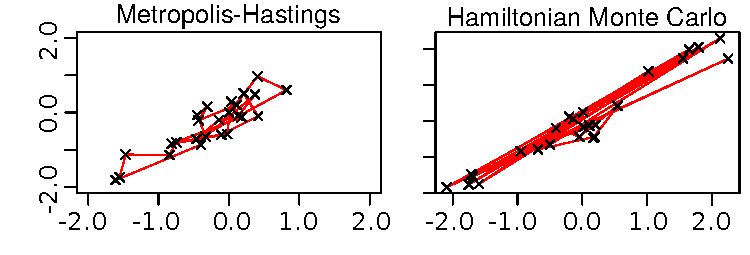
\includegraphics[width=5in]{images/MHvsHM_explore.pdf}
\caption{The trajectory of a bivariate Gaussian distribution simulated with zero-mean and marginal $\sigma$ of 1, and $\rho$ of 0.95.}
\end{figure}


\begin{figure}[H]
\center
  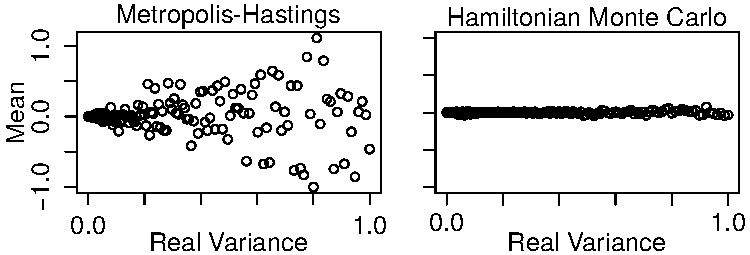
\includegraphics[width=5in]{images/MHvsHM_var.pdf}
  \caption{Mean}
\end{figure}
\subsection{High-dimensionality}
\begin{figure}[H]
\center
  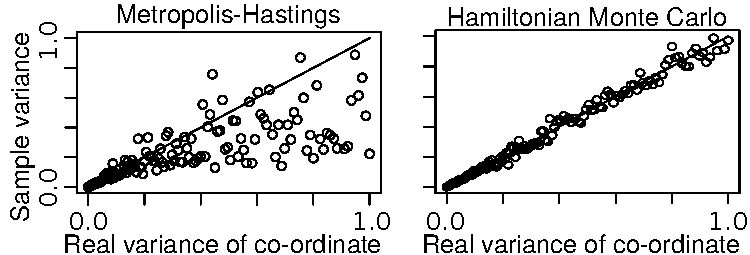
\includegraphics[width=5in]{images/MHvsHM_varcoord.pdf}
  \caption{A comparison of the real and observed variance of a highly-dimensional mutivariate Gaussian.}
\end{figure}
\subsection{Choices of $\epsilon$ and L}


\subsection{No U-turn sampler (NUTS)}
The No U-turn sampler\cite{NUTS} is an implementation of Hamiltonian Monte Carlo which aims to avoid the need for the user to manually specify $L$ and $\epsilon$
\cite{rstan}
\subsection{Normal mixture models}
We compared the performance of our model to that of the Metropolis-Hastings algorithm and the NUTS method, as implemented in RStan

\begin{thebibliography}{9}

\bibitem{neal}
  Neal R.M.,
  \emph{MCMC using Hamiltonian dynamics},
  Chapter 5 of the Handbook of Markov Chain Monte Carlo,
  2012.
  
\bibitem{duane}
  Duane,S., Kennedy,A.D., Pendleton,B.J., \& Roweth,D.,
  \emph{Hybrid Monte Carlo }
  Physics Letters B, 195(2) 216-222, 1987.

\bibitem{NUTS}
  Hoffman,M.D., Gelman,A.,
  arXiv:1111.4246v1.
  
\bibitem{rstan}
  RStan, \url{http://mc-stan.org/interfaces/rstan.html}

\end{thebibliography}
\end{document}
